% Harus dimuat terlebih dahulu, digunakan agar file PDF memiliki format karakter yang benar.
% Untuk informasi lebih lanjut, lihat https://ctan.org/pkg/cmap.
\RequirePackage{cmap}

% Format dokumen sebagai paper konferensi menggunakan aturan IEEEtran terbaru (v1.8b).
% Untuk informasi lebih lanjut, lihat http://www.michaelshell.org/tex/ieeetran/.
\documentclass[conference]{IEEEtran}[2015/08/26]

% Format encoding font dan input menjadi 8-bit UTF-8.
\usepackage[T1]{fontenc}
\usepackage[utf8]{inputenc}

% Format bahasa menjadi bahasa german dan inggris.
\usepackage[english]{babel}

% Digunakan untuk tujuan demonstrasi.
\usepackage{mwe}

% Digunakan untuk menampilkan font dengan style yang lebih baik.
\usepackage[zerostyle=b,scaled=.75]{newtxtt}

% Digunakan untuk menampilkan tabel dengan style yang lebih baik.
\usepackage{booktabs}

% Digunakan untuk menampilkan gambar pada dokumen.
\usepackage{graphicx}

% Digunakan untuk menampilkan potongan kode.
\usepackage{listings}
\lstset{
  basicstyle=\ttfamily,
  columns=fixed,
  basewidth=.5em,
  xleftmargin=0.5cm,
  captionpos=b
}

% Digunakan agar backticks (`) dapat dirender pada PDF.
% Untuk informasi lebih lanjut, lihat https://tex.stackexchange.com/a/341057/9075.
\usepackage{upquote}

% Digunakan untuk menyeimbangkan bagian akhir dokumen dengan dua kolom.
\usepackage{balance}

% Digunakan untuk menampilkan pustaka.
\usepackage[square,comma,numbers,sort&compress]{natbib}

% Mengubah format ukuran teks pada natbib.
\renewcommand{\bibfont}{\normalfont\footnotesize}

% Menambah nama penulis ketika menggunakan perintah \citet.
% Untuk informasi lebih lanjut, lihat https://tex.stackexchange.com/a/76075/9075.
\usepackage{etoolbox}
\makeatletter
\patchcmd{\NAT@test}{\else \NAT@nm}{\else \NAT@hyper@{\NAT@nm}}{}{}
\makeatother

% Digunakan untuk melakukan linewrap pada pustaka dengan url yang panjang
% jika terdapat hyphens
\usepackage[hyphens]{url}

% Digunakan untuk menambah hyperlink pada referensi.
\usepackage{hyperref}

% Menonaktifkan warna dan bookmark pada hyperref.
\hypersetup{hidelinks,
  colorlinks=true,
  allcolors=black,
  pdfstartview=Fit,
  breaklinks=true
}

% Digunakan untuk membenarkan hyperref pada gambar.
\usepackage[all]{hypcap}

% Digunakan untuk menampilkan beberapa gambar
\usepackage[caption=false,font=footnotesize]{subfig}

\usepackage{stfloats}

% Tambahkan format tanda hubung yang benar di sini
\hyphenation{
  ro-ket
  me-ngem-bang-kan
  per-hi-tu-ngan
}

\begin{document}

  % Ubah kalimat berikut sesuai dengan judul penelitian.
\title{Retrieval Augmented Generated Chatbot for Earth Fault Simulation}

% Ubah kalimat-kalimat berikut sesuai dengan nama, institusi, alamat dan kontak penulis.
\author{
  \IEEEauthorblockN{Farid Cenreng}
  \IEEEauthorblockA{Department of Computer Engineering\\
  Faculty of Intelligent Electrical and Informatics Technology\\
    Institut Teknologi Sepuluh Nopember\\
    Surabaya, Indonesia 60111\\
    5024201005@students.its.ac.id}

  \and
  \IEEEauthorblockN{Supeno Mardi Susiki Nugroho}
  \IEEEauthorblockA{Department of Computer Engineering\\
  Faculty of Intelligent Electrical and Informatics Technology\\
    Institut Teknologi Sepuluh Nopember\\
    Surabaya, Indonesia 60111\\
    mardi@its.ac.id}

  \and
  \IEEEauthorblockN{Reza Fuad Rachmadi}
  \IEEEauthorblockA{Department of Computer Engineering\\
  Faculty of Intelligent Electrical and Informatics Technology\\
    Institut Teknologi Sepuluh Nopember\\
    Surabaya, Indonesia 60111\\
    fuad@its.ac.id}
}

% Digunakan untuk menampilkan judul dan deskripsi penulis.
\maketitle

  % Mengubah keterangan `Abstract` ke bahasa indonesia.
% Hapus bagian ini untuk mengembalikan ke format awal.
\renewcommand\abstractname{Abstrak}

\begin{abstract}

  % Ubah paragraf berikut sesuai dengan abstrak dari penelitian.
  Pemecahan masalah kelistrikan kapal tetap merupakan proses yang menantang dan membutuhkan banyak latihan, sehingga diperlukan media pembelajaran simulasi yang melatih pelajar untuk mengatasi masalah kelistrikan. Pelajar tentunya membutuhkan bimbingan selama pelatihan untuk memperoleh hasil yang maksimal. Bimbingan konvensional berupa diskusi dengan pembimbing, tentunya tidak efektif karena akan sangat dibatasi oleh waktu dan sumber daya. Diusulkan penggunaan \emph{chat bot} untuk menyediakan media bertanya dan konsultasi efektif untuk menyelesaikan kendala kelistrikan pada kapal, dengan menggunakan \emph{ Natural Language Understanding} (NLU), untuk
  dapat mengerti intensi dari pertanyaan secara tepat. \emph{Chat bot} dirancang untuk membantu peserta dalam registrasi dan penggunaan simulasi. Selain itu, chat bot juga dirancang untuk membantu peserta memahami \emph{Earth Fault} secara detail. Dengan adanya \emph{chat bot}, peserta pelatihan dapat berkonsultasi tanpa terbatas oleh waktu kerja dan zona waktu.
\end{abstract}

% Mengubah keterangan `Index terms` ke bahasa indonesia.
% Hapus bagian ini untuk mengembalikan ke format awal.
\renewcommand\IEEEkeywordsname{Kata kunci}

\begin{IEEEkeywords}

  % Ubah kata-kata berikut sesuai dengan kata kunci dari penelitian.
  Natural Language Understanding, Chat Bot, Earth Fault, Simulasi.

\end{IEEEkeywords}


  % Ubah bagian berikut sesuai dengan konten-konten yang akan dimasukkan pada dokumen
  % Ubah judul dan label berikut sesuai dengan yang diinginkan.
\section{Pendahuluan}
\label{sec:pendahuluan}

% Ubah paragraf-paragraf pada bagian ini sesuai dengan yang diinginkan.

Pemecahan masalah kelistrikan kapal tetap merupakan proses yang membutuhkan banyak latihan dan pengalaman teknis. Untuk memberi pengalaman teknis ini, perlu dilakukan pelatihan sercara langsung diatas kapal. Namun, tidak semua institusi mampu menyediakan kapal yang diperlukan untuk melatih pelajar
. Untuk membantu proses pelatihan ini, telah dilakukan penelitian oleh Ibu Rona Riantini yang mengusulkan permainan simulasi sebagai media pembelajaran \cite{riantini2022serious}. Untuk menyediakan pelatihan yang lebih efektif, diusulkan penggunaan \emph{chat bot} untuk membantu peserta dalam registrasi dan penggunaan simulasi. Selain itu, \emph{chat bot} juga  dirancang untuk membantu peserta memahami \emph{Earth Fault} secara detail. \emph{Chat bot} dengan menggunakan media website dalam operasinya. \emph{Chat bot} adalah sistem yang digunakan untuk merespon pertanyaan yang diberikan pengguna dengan dengan menggunakan bahasa mereka \cite{9501523}. Penggunaan \emph{chat bot} akan diimplementasikan dengan \emph{Natural Language Processing} (NLP),  untuk menghasilkan pengenalan bahasa yang lebih bagus. NLP adalah cabang dari kecerdasan buatan yang fokus pada pemahaman dan penghasilan teks atau bahasa manusia oleh komputer. \emph{Chat bot} yang menggunakan NLP memiliki kemampuan untuk memahami, memproses, dan merespons teks atau ucapan manusia secara otomatis \cite{9402401}. NLP sendiri memiliki kelemahan pada terbatasnya informasi yang dimiliki. NLP hanya dapat mengakses informasi yang diberikan pada saat proses pelatihan. Oleh karena itu, diperlukan sistem \emph{Retrieval Augmented Generation} (RAG). RAG memungkinkan LLM untuk mengambil data eksternal berupa dokumen, dataset, bahkan akses internet. Untuk dapat mengerti data yang diberikan, harus dilakukan proses \emph{embeddings} pada RAG untuk memperoleh makna dari data. Untuk mengatasi dokumen besar, dilakukan metode \emph{chunking} untuk mebagi dokumen menjadi lebih kecil agar mempermudah proses pencarian informasi. Setelah memperoleh informasi yang relevan, informasi akan diolah oleh NLP menjadi jawaban untuk pertanyaan pengguna \cite{10448015}. Sistem akan dibuat dalam bentuk website, dan akan dihubungkan dengan website simulasi \emph{earth fault}. Sistem dirancang untuk memberi interaksi natural pada pengguna. Sistem ini diharapkan bisa menjadi sarana tanya jawab untuk membantu pengguna dalam menggunakan sistem simulasi, dan juga untuk membantu pengguna memahami konsep \emph{earth fault} secara mendalam. 

Pembahasan pada paper ini dimulai dengan presentasi mengenai penelitian lain (Bagian \ref{sec:penelitianterkait}).
Kemudian dilanjutkan dengan penjelasan mengenai arsitektur dari sistem yang dibuat (Bagian \ref{sec:arsitektur}).
Berdasarkan hal tersebut, kami menunjukkan hasil yang diperoleh dari sistem yang dibuat(Bagian \ref{sec:loremipsum}).
Terakhir, didapatkan kesimpulan dari penelitian yang telah dilakukan (Bagian \ref{sec:kesimpulan}).

  % Ubah judul dan label berikut sesuai dengan yang diinginkan.
\section{Related Research}
\label{sec:penelitianterkait}

% Ubah paragraf-paragraf pada bagian ini sesuai dengan yang diinginkan.
\subsection{Impact of chat bots usage in learning}
Research by Ms. Rona Riantini, which proposed simulation games as a learning medium, emphasizes the importance of effectively addressing problems on ships. Incorrect or slow handling can result in significant losses and even casualties. To train problem-solving skills, training for prospective crew members through electrical fault simulations on ships is necessary \cite{riantini2022serious}. This learning requires continuous practice and also needs adaptive feedback to effectively enhance student capabilities. Therefore, a teacher's presence is needed to guide students in understanding issues and directing problem-solving. However, the presence of teaching staff is less effective due to limitations in time and place. Many educators are needed to personally guide each student. Therefore, integrating a \emph{chatbot} as a guidance tool in the simulation of solving electrical problems on ships can offer significant benefits. With the \emph{chatbot}, consultation and guidance services can be provided to many students and can be conducted anytime. With the \emph{chatbot}, learning can be personalized for each student. Learning can adapt to the pace and learning style of each individual effectively and flexibly \cite{vazquezcano2021chatbot,kumar2021educational}. In research conducted by Essel, the performance of students at the University of Ghana trained by a \emph{chatbot} and those trained by an instructor was tested. From the results obtained, students interacting with the \emph{chatbot} showed better performance compared to the control group that interacted with a course instructor. Students trained by the \emph{chatbot} achieved an average score of 81.1, while those trained by an instructor scored 65.2. Students also felt very satisfied with the use of the chatbot, especially because it could provide instant feedback without delays in the interaction process \cite{essel2022virtual}.


\subsection{Related research on Retrieval Augmented Generation (RAG) method}
The \emph{Retrieval Augmented Generation} (RAG) technology enhances the answer generation capabilities of \emph{Large Language Models} (LLM) to be more accurate and relevant by integrating content retrieved from an external knowledge base to respond to user prompts \cite{xu2024nanjing}. This system is an advancement over previous systems that used \emph{Rule-Based} systems, meaning that users could only access the system by following a specific set of rules \cite{9501523}. This system was developed to address the rigid and limited shortcomings of the previous method. The \emph{chatbot} uses the LLM system to provide more natural answers, unlike instruction-based systems that are limited to specific instructions given by the user \cite{sarrouti2020sembionlqa}. RAG enables LLM to pull external data such as documents, datasets, and even internet access. This allows for taking a user's question, searching it from a data source, and then processing it into a natural response for the user \cite{tian2023intelligent}. To understand the provided data, an \emph{embeddings} process must be conducted on RAG to derive meaning from the data. To manage large documents, a \emph{chunking} method is used to divide the document into smaller parts to facilitate the information search process \cite{10448015}.


The system developed in this study includes several stages. First, words from external data sources and words from user prompts are converted into word vectors. For this, the concept of \emph{vector embedding} is used, which represents numerical vectors of data typically used to describe words, phrases, or even documents in a vector space \cite{kmetty2021presence}. In the concept of \emph{Neural Networks}, \emph{embedding} is a low-dimensional data representation that captures essential aspects of the original data. The concept of \emph{embedding} is widely used in language processing and recommendation systems. The main goal of \emph{embedding} is to transform non-numeric data, such as words or items, into numeric vectors so that computer \emph{neural network} systems can process them. One of the main advantages of \emph{embedding} is its ability to capture semantic relationships between data. In \emph{embedding} processing, words with similar contexts will have similar vector representations \cite{luo2018concept}.


Afterwards, the vectorized data is stored in a vector database with the assistance of the \emph{Facebook AI Similarity Search (FAISS)}, which creates vector indexes and uses an efficient and accurate nearest neighbor search algorithm for data retrieval \cite{10039758}. The FAISS algorithm utilizes the \emph{Product Quantization} (PQ) method, a technique for compressing high-dimensional data vectors into shorter, more efficient codes for storage and data retrieval. The article "A Survey of Product Quantization" explains that the PQ process involves dividing the input vector into smaller sub-vectors, each of which is then quantized independently. Each sub-vector is encoded into a specific identification from these independent parts, and these identifications are combined to form a PQ code that represents the original vector. One of the main advantages of PQ is its ability to efficiently estimate the distance between the original vector and its PQ code using \emph{Asymmetric Distance Computation} (ADC). This method allows for fast searching within very large databases using a \emph{lookup table}. Subsequently, the data retrieval results and user prompts are input into the LLM model to generate a more accurate final answer. The RAG method integrates the retrieval model and LLM, extracts semantic features from questions and answers, and ranks results based on semantic relevance between texts, then inputs the retrieval results into a large language model for enhanced generation, thus achieving a knowledge-based smart question answering system.





% Beberapa penelitian lain pernah dilakukan seperti yang dirumuskan oleh \citet{newton1687} bahwa \lipsum[5]
% Hasil tersebut kemudian menjadi persamaan \ref{eq:hukumpertama}.

% % Contoh pembuatan persamaan ilmiah.
% \begin{equation}
%   \label{eq:hukumpertama}
%   \sum \mathbf{F} = 0\; \Leftrightarrow\; \frac{\mathrm{d} \mathbf{v} }{\mathrm{d}t} = 0.
% \end{equation}


  % Ubah judul dan label berikut sesuai dengan yang diinginkan.
\section{Architecture}
\label{sec:arsitektur}

% Ubah paragraf-paragraf pada bagian ini sesuai dengan yang diinginkan.

\subsection{Retriever}
\label{subsec:Retriever}

Before using data for the language model, it is necessary to search for relevant data. To perform this data search, searches are conducted by looking at the location of the data within the vector. For this, data must be converted into a vector format that can be computed. There are many methods for doing this, such as \emph{one-hot}, \emph{Word2Vec}, and \emph{Doc2Vec}. These methods provide effective pathways for text quantification but often ignore contextual information. The \emph{Transformer} model, introduced by Google in 2017, overcomes the shortcomings of existing text quantification methods and is built using unsupervised training on large volumes of unlabeled corpus data \cite{vaswani2017attention}. The \emph{Transformer} is a neural network architecture widely used in NLP, text classification, question-answering systems, and more. This model consists of several \emph{encoders} and \emph{decoders}, each composed of several layers of identical blocks. These blocks are stacked together to form the overall \emph{Transformer} architecture \cite{miao2016processing}. The structure of the \emph{transformer} can be seen in Figure \ref*{fig:transformer}.

\begin{figure*}
  \centering
  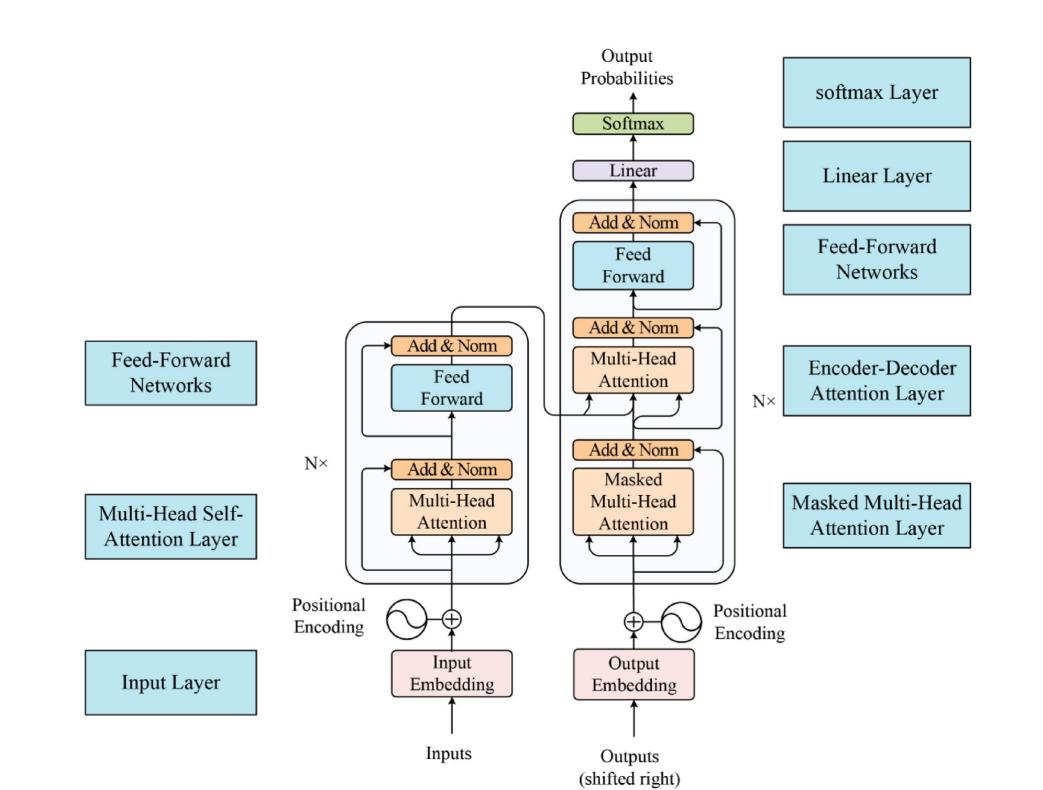
\includegraphics[width=.6\textwidth]{gambar/struktur-transformer.jpg}
  \caption{Transformer structure \cite{vaswani2017attention}}
  \label{fig:transformer}
\end{figure*}

In the \emph{transformer} architecture, there are two main components: the \emph{encoder} and the \emph{decoder}, each consisting of a series of identical layers. Each layer in the \emph{encoder} and \emph{decoder} has two sub-layers, namely the \emph{multi-head attention} mechanism and the \emph{fully connected network}. \emph{Multi-head attention} allows the model to process parts of the data in parallel and integrate information from various positions within the data. Furthermore, the \emph{transformer} features a \emph{self-attention} mechanism, which allows each output from the \emph{encoder} or \emph{decoder} to consider all previous inputs. This differs from other algorithms that are limited by the distance between relevant inputs and outputs. This mechanism also aids in understanding long-term dependencies in text, which is crucial for tasks such as translation. \emph{Positional encoding} is used to provide positional information to the model, as the \emph{transformer} model lacks recursion or convolution that naturally captures the sequence of information \cite{vaswani2017attention}.
 

\subsection{Augment and Generation}
\label{subsec:AugmentGeneration}

During the \emph{augmentation} process, the LLM model will operate by processing the \emph{prompt} from the user using the context already obtained from the previous \emph{retriever} process \cite{bansal2024llm}. The tool is implemented by first creating a backend system using LangChain to connect various modules and LLM processes. LangChain serves as a connector to various other modules. Subsequently, a selection of the LLM framework to be used is made. The framework employed must be \emph{open-source} and lightweight in order to be effective in use. Therefore, in the testing phase, trials will be conducted on various frameworks to test the effectiveness of these frameworks. Some to be tested include RASA, Hugging Face, and Ilama Cpp. Testing is conducted by evaluating the performance of each framework, as well as considering their advantages and disadvantages. After that, the most effective framework will be selected for use in implementing this tool.

During the \emph{generation} process, the LLM model will produce output in the form of answers to the questions provided by the user. This output will be given to the user as an answer to their question. In this process, the LLM model will utilize the context obtained from the previous \emph{retriever} process. Thus, the LLM model will be able to provide answers that are more relevant and accurate. The testing used the following configuration:
\begin{lstlisting}[
  language=python,
  caption={Test configuration},
]
model = AutoModelForCausalLM.from_pretrained(
   "$MODEL_NAME",
    load_in_8bit=True,
)
pipeline = pipeline(
    "text-generation",
    model=model,
    return_full_text=False,
    tokenizer=tokenizer,
    max_new_tokens=512,
     do_sample=True,
    pad_token_id=tokenizer.eos_token_id
)
\end{lstlisting}

After that, an analysis is conducted on the results obtained from the LLM model. The results will be analyzed based on the relevance and accuracy of the answers provided. This is done by comparing the answers with the answers from the data source. For example, for the question: "What should be done in the event of a power outage?" the relevant answer according to the book is "In the event of a power outage, do not panic, the emergency generator will restore power shortly, find out the problem and reason for the power outage, inform the authorities...". Furthermore, an analysis is conducted on the use of RAM and VRAM. This is done to determine how efficient the LLM model is in using resources. Thus, it can be determined how effective the LLM model is in providing answers that are relevant, accurate, and efficient.


% Contoh input gambar pada kolom.
% \begin{figure} [ht]
%   \centering
%   % Ubah sesuai dengan nama file gambar dan ukuran yang akan digunakan.
%   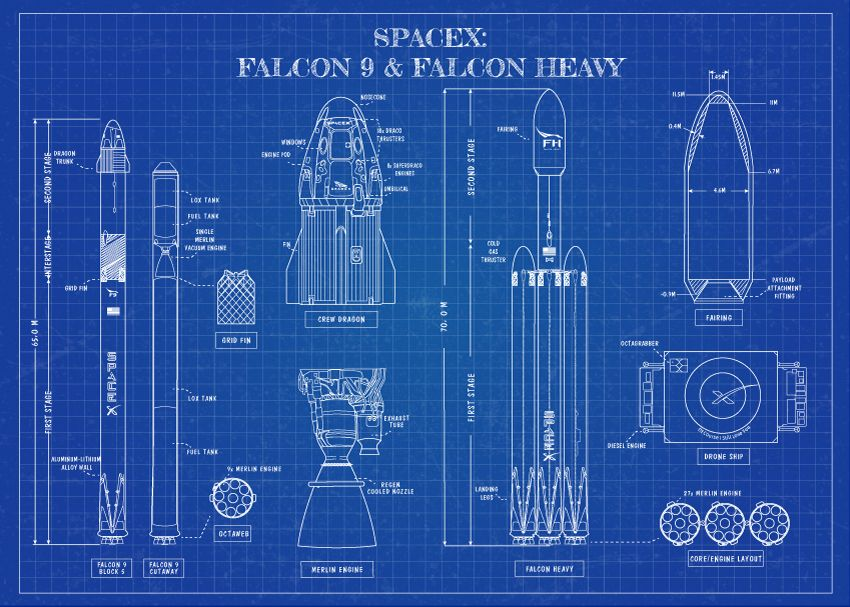
\includegraphics[width=0.4\textwidth]{gambar/cetakbiru.jpg}

%   % Ubah sesuai dengan keterangan gambar yang diinginkan.
%   \caption{Cetak biru roket yang akan diuji coba. \cite{cetakbiruspacex}}
%   \label{fig:cetakbiru}
% \end{figure}

% \lipsum[9-10]

% \subsection{Lorem Ipsum}
% \label{subsec:loremipsum}

% \lipsum[11]

% % Contoh pembuatan tabel.
% \begin{table}
%   \caption{Contoh tabel sederhana}
%   \label{tab:tabelsederhana}
%   \centering
%   \begin{tabular}{lll}
%     \toprule
%     Heading1 & Heading2 & Heading3  \\
%     \midrule
%     One      & Two      & Three     \\
%     Four     & Five     & Six       \\
%     \bottomrule
%   \end{tabular}
% \end{table}

% % Contoh pembuatan potongan kode.
% \begin{lstlisting}[
%   language=C++,
%   caption={Program halo dunia.},
%   label={lst:halodunia}
% ]
% #include <iostream>

% int main() {
%     std::cout << "Halo Dunia!";
%     return 0;
% }
% \end{lstlisting}

% \lipsum[12]

% % Contoh pembuatan daftar.
% \begin{enumerate}
%   \item \lipsum[13][1-4]
%   \item \lipsum[13][5-8]
%   \item \lipsum[13][9-12]
% \end{enumerate}

% \lipsum[14-15]

  % Ubah judul dan label berikut sesuai dengan yang diinginkan.
\section{Results}
\label{sec:analisahasil}

After the text has done, the results obtained from the LLM model will be analyzed. The results obtained will be analyzed based on how much resources it uses. Results also evaluated by the relevance and accuracy of the answers given. 

\subsection{RASA Framework}
The first is testing using the \emph{RASA} framework. From this testing, it was found that RASA has advantages in terms of easy \emph{deployment}. However, RASA has shortcomings in terms of \emph{training}. RASA conducts \emph{training} using existing data. RASA uses YAML files to store its configurations. These configurations must contain the data to be used. Conversations will be limited to this existing data. This causes RASA to be unable to respond to questions outside this data. If users provide input different from the data, RASA will struggle to understand the user's intent. This results in RASA being unable to provide answers that match the user's questions. RASA can be used effectively if the user has an extensive question and answer dataset so that RASA can provide appropriate answers. This constraint significantly hinders RASA’s ability to handle queries or interactions that deviate from the predefined datasets. When faced with unfamiliar user inputs, RASA often struggles to accurately interpret the user's intent, leading to responses that do not align with the user's actual questions or needs. While RASA can be effective when a comprehensive dataset of questions and answers is available, this necessity limits its flexibility and scalability.

RASA also lacks an active community, which means the development of RASA is slower compared to other \emph{frameworks}. RASA’s development suffers from a lack of robust community support. Unlike platforms such as \emph{HuggingFace}, which thrive on active community contributions and continuous advancements, RASA's community is relatively inactive. This lack of engagement results in slower updates and enhancements, contributing to RASA being perceived as outdated compared to more dynamic and community-driven frameworks. The culmination of these factors makes RASA a less optimal choice for deployment in projects that demand adaptability and ongoing development support. This causes RASA to be less optimal for use in this project.

The creation of a \emph{chatbot} using the Llama.cpp \emph{framework} with the aya-23-8B-Q4-K-M model requires 3.3 GB of RAM and 5.1 GB of VRAM, and takes 6 seconds to process a response. The resulting \emph{chatbot} has a \emph{Faithfulness} score of 93.095\%, an \emph{Answer Relevancy} score of 98.299\%, and an \emph{Answer Correctness} score of 77.093\%. Next, testing was conducted using RAGAs to evaluate the overall performance of RAG. This involved testing the aya-23-8B-Q4-K-M model used in the final results. The test consisted of 75 questions created and answered by humans. These questions were then also answered by the RAG model, and the answers were compared to the human answers. The metrics assessed in this testing included Faithfulness, Answer Relevancy, and Answer Correctness. This evaluation allowed for a detailed comparison between the human-generated answers and those provided by the \emph{chatbot}, highlighting the model's strengths and areas for improvement. 
\subsection{Langchain and HuggingFace Framework }
The next is testing using a combination of LangChain and HuggingFace. From the test results obtained in Table  \ref{tab:hasilrag}
\begin{table}[!htbp]
  \caption{Langchain and HuggingFace results}
  \label{tab:hasilrag}
  \centering
  \begin{tabular}{llll}
    \toprule
    Name                      & R/V(GB) & T(s)  & Result \\
    \midrule
    bigscience/bloom-7b1      & 2.5/8.2    &27   & Accurate, but \\ \cite{muennighoff2022crosslingual}                          &          &           & not natural \\  
    \\
    bigscience/bloom-1b7
    \cite{muennighoff2022crosslingual}      & 3.1/6.9   &15    & Accurate, but \\
                              &          &           & not natural \\ 
    \\ 
    sail/Sailor-4B \cite{dou2024sailor}           & 4.3/6.3    &20   & Inaccurate \\
    \\
    sail/Sailor-0.5B \cite{dou2024sailor}          & 2.3/2.7   &12    & Inaccurate \\
    \\
    indonlp/cendol-mt5-       & 3.0/0.7  &22     & Accurate, but \\
    small-inst \cite{indonlp1,indonlp2, indonlp3, indonlp4, indonlp5, indonlp6, indonlp7}              &          &           & not natural \\ 
    \\
    indonlp/cendol-llama2-    & 2.5/0.7   &25      & Inaccurate \\
    7b-chat \cite{indonlp1,indonlp2, indonlp3, indonlp4, indonlp5, indonlp6, indonlp7}                  &          &           &  \\
    \\
    Yellow-AI-NLP/komodo-     & 5.0/7.3   &30    & Inaccurate \\
    7b-base \cite{owen2024komodo}                  &          &           &  \\
    \\
    cahya/gpt2-small-         & 2.4/0.4   &11    & Inaccurate \\
    indonesian-522M \cite{cahya_llm}          &          &           &  \\
    \\
    kalisai/Nusantara-7b-     & 3.2/9.9   &19    & Accurate, but \\
    Indo-Chat \cite{zulfikar_aji_kusworo_2024}        &          &           & not natural \\
    \\
    kalisai/Nusantara-4b-     & 4.4/6.3   &12    & Accurate, but \\
    Indo-Chat  \cite{zulfikar_aji_kusworo_2024}               &          &           & not natural \\
    \bottomrule
  \end{tabular}
\end{table}


\subsection{Framework Langchain dan Llama.cpp}
Next is testing using a combination of LangChain and Llama.cpp. From the test results obtained in Table \ref{tab:hasilllama}
\begin{table}[!htbp]
  \caption{llama.cpp Results}
  \label{tab:hasilllama}
  \centering
  \begin{tabular}{llll}
    \toprule
    Name                      & R/V(GB) & T(s)  & Result \\
    \midrule
    bigscience/bloom-7b1      & 2.5/8.2    &18   & Accurate, but \\ \cite{muennighoff2022crosslingual}                          &          &           & not natural \\  
    \\
    bigscience/bloom-1b7
    \cite{muennighoff2022crosslingual}      & 3.1/6.9   &15    & Accurate, but \\
                              &          &           & not natural \\ 
    \\ 
    Merak-7B-v4-model-Q4 \cite{Merak}       & 3.4/5.3    &13   & Accurate, but \\
                              &          &           & not natural \\
    \\
    Merak-7B-v4-model-Q5 \cite{Merak}       & 3.5/6.0   &15    & Accurate, but \\
                              &          &           & not natural \\
    \\
    aya-23-8B-Q6-K \cite{aryabumi2024aya}   & 3.3/7.0  &10     & Accurate \\
    \\
    aya-23-8B-Q4-K-M \cite{aryabumi2024aya} & 3.3/5.1   &6      & Accurate, but \\
                              &          &           & not optimal \\
    \bottomrule
  \end{tabular}
\end{table}

\subsection{Overall Testing with RAGAs}

To observe overall performance of RAG process. This experiment utilized the RAGAs framework, specifically testing the model aya-23-8B-Q4-K-M. We tested the model by comparing its responses to 75 human-answered questions across metrics such as Faithfulness, Answer Relevancy, and Answer Correctness.
To test the RAG pipeline is challenging because the RAG pipeline consists of several different components to be tested. When evaluating the RAG pipeline, both components must be evaluated separately but simultaneously to understand if and where the RAG pipeline still needs improvement. RAGAs is a framework that allows easy evaluation of RAG \cite{es2023ragas}. RAGAs evaluate the results of RAG by creating a dataset, which is then supplemented with answers from the RAG model. This dataset consists of four parts:

\begin{enumerate}[nolistsep]
\item \emph{Question}: A list of questions to be tested on the model. These questions can be manually created by humans or generated using synthetic features available in RAGAs.
\item \emph{Ground truths}: The correct answers to the questions. This section can also be created by humans or generated synthetically. This information is essential for the \emph{context recall} metric.
\item \emph{Answer}: The responses produced by the RAG pipeline. This is the output from the tested RAG model.
\item \emph{Contexts}: The context retrieved from external knowledge sources used to answer the questions.
\end{enumerate}

Using this dataset, RAGAs then evaluates the results of the RAG model.
The first test used a bi-encoder for the retriever. The results showed a Faithfulness score of 45.415\%, an Answer Relevancy score of 88.965\%, and an Answer Correctness score of 54.193\%. These scores indicated that the generated answers were lacking in Faithfulness and Answer Correctness, meaning the answers were far from factual. This was attributed to the context not matching the given questions, causing the model to respond without using the entire or correct context, leading to low scores in Faithfulness and Answer Correctness.

The second test used a cross-encoder for the retriever, as cross-encoders provide better results with a small data source, though they take longer to process information compared to bi-encoders. This test yielded a Faithfulness score of 79.931\%, an Answer Relevancy score of 96.236\%, and an Answer Correctness score of 62.596\%. These scores showed improved answers in all aspects. However, the Faithfulness and Answer Correctness scores still did not reach the desired levels. This was due to the context being truncated by the system's method of dividing data into smaller pieces with TextSplitter.

The third test used the same configuration as the second but divided the data differently, grouping sections by context. This test resulted in a Faithfulness score of 86.269\%, an Answer Relevancy score of 96.536\%, and an Answer Correctness score of 65.196\%. These scores showed further improvements in all aspects, though the Faithfulness and Answer Correctness scores still fell short of the desired levels. This was because the generated answers were longer than necessary, influenced by the model's high temperature setting, which caused it to provide more detailed explanations. Additionally, the model was prompted to explain its answers, resulting in longer responses.

The fourth test also used the same configuration as the third but with a lower temperature setting and a prompt for concise yet detailed answers. This test produced a Faithfulness score of 93.095\%, an Answer Relevancy score of 98.299\%, and an Answer Correctness score of 77.093\%. These results indicated significant improvements in all aspects, though the Answer Correctness score still did not reach 90\%. However, considering that these scores were compared to human answers, the results were deemed satisfactory.

A comparison table of all the test results can be seen in Table \ref{tab:hasilragas}, which displays the Faithfulness, Answer Relevancy, and Answer Correctness scores for each test conducted.

Results from all tests are compiled in Table \ref{tab:hasilragas}, with Faithfulness (F), Answer Relevancy (AR), Answer Correctness (AC).


\begin{table}[!htbp]
  \caption{RAGAs Results}
  \label{tab:hasilragas}
  \centering
  \begin{tabular}{llll}
    \toprule
    No & F (\%) & AR (\%) & AC {\%} \\
    \midrule
    1& 45,415  & 88,965 & 54,193 \\
    2& 79,931 & 96,236 & 62,596 \\
    3& 86,269 & 96,536 & 65,196 \\
    4& 93,095 & 98,299 & 77,093 \\
    \bottomrule
  \end{tabular}
\end{table}
% Ubah paragraf-paragraf pada bagiaOveran ini sesuai dengan yang diinginkan.

% % Contoh input beberapa gambar pada halaman.
% \begin{figure*}
%   \centering
%   \subfloat[Hasil A]{\includegraphics[width=.4\textwidth]{example-image-a}
%     \label{fig:hasila}}
%   \hfil
%   \subfloat[Hasil B]{\includegraphics[width=.4\textwidth]{example-image-b}
%     \label{fig:hasilb}}
%   \caption{Contoh input beberapa gambar.}
%   \label{fig:hasil}
% \end{figure*}

% \lipsum[16-18]

% % Contoh input potongan kode dari file.
% \lstinputlisting[
%   language=Python,
%   caption={Program perhitungan bilangan prima.},
%   label={lst:bilanganprima}
% ]{program/bilangan-prima.py}

% \lipsum[19-20]

  % Ubah judul dan label berikut sesuai dengan yang diinginkan.
\section{Conclusion}
\label{sec:kesimpulan}

% Ubah paragraf-paragraf pada bagian ini sesuai dengan yang diinginkan.

From the experiments conducted, it can be concluded that creation of chatbot using the Llama.cpp framework can be achieved and produces satisfying responses. This specifically with the aya-23-8B-Q4-K-M model, that has shown significant improvements in response quality when tested with 75 human-answered questions. The results of the tests showed that the model's reach Faithfulness of 93,095\%, Answer Relevancy of 98,299\%, and Answer Correctness of 77,093\% while only using 5,1 GB of VRAM and take about 6s to generate answer.

  % Menampilkan daftar pustaka dengan format IEEE
  \bibliographystyle{IEEEtranN}
  \bibliography{pustaka/pustaka.bib}

  % Menyeimbangkan bagian akhir di kedua kolom
  \balance

\end{document}
